\documentclass{article}
\title{Hand Written Digit Recognition using Convolutional Neural Network (CNN)}\author{Kavitha Konduru}
\usepackage{graphicx}
\graphicspath {{figures/}}
%ref{•}
%\usepackage{cite}
\usepackage{natbib} 
\usepackage{hyperref}
\usepackage{url}

\begin{document}

\maketitle

\begin{abstract}
  Recent advancements in digital image processing and machine learning have enabled a rapid development of new face recognition techniques. A goal of this study is to extend these approaches for developing machine learning techniques that recognize handwritten characters from complex images. A specific objective was to develop and implement a convolution neural network (CNN) model for recognizing handwritten digits from an image. A large dataset from the Modified National Institute of Standards and Technology (MNIST) database was used to evaluate the performance of the CNN model. Convolutional neural networks (convNets) are a special type of feedforward neural networks (NN). The model was further predicted using the author generated hand-written images. The developed model compared the ‘SoftMax’ and ‘Sigmoid’ activation results. We used the relevant techniques for establishing the accuracy and precision of the model. Preliminary results suggest that the neural network modeling framework developed in this study could be used to recognize bacteria from an image of a complex biological film. 
\end{abstract}

\section{Introduction}

\paragraph{•}
HANDWRITTEN digit recognition technologies enable an automated method for recognizing handwritten characters from documents such as emails, papers, images, and business letters [1]. The digit recognition technologies can be found in applications related to signature verification, bank check processing, and postal address interpretation from envelopes [2]. The digit recognition techniques based on machine learning techniques have used classification systems such as K-nearest Neighbors, SVM classifier, and Random Forest Classifier and CNN. Compared to these models, the CNN has been reported to yield accurate results [2]. It is clear that the CNN models are beneficial for real world applications. For example, a prior study has reported that the typical machine learning techniques implemented for postal delivery application failed to distinguish two similarly spelled first names (e.g., “Anuj” vs. “Tanuj”). This error resulted in delivery of the post to a wrong person [2]. Some of these limitations associated with inaccurate interpretations could be alleviated by using deep learning techniques, especially using CNN techniques for image processing, object detection, and handwritten digit and character recognition [3]. 

\paragraph{•}
CNNs use a variation of multilayer perceptrons designed to require minimal preprocessing [2].CNN models have been reported to present powerful tools for enhancing the fields of signal and image processing as well as computer vision that deals with handwriting recognition, natural object classification and segmentation. Examples of deep learning API frameworks developed in python include Pybrains, Keras, Theano, Tensorflow etc. 
\paragraph{•}
Based on the above background, a goal of this study was to develop a handwriting recognition system that processes a given picture and recognizes handwritten digits using MNIST pretrained labels and Keras APIs. The deep learning model features mechanisms for extracting the features of the hand written digits. We have used  the supervised classification algorithm CNN to train the model and compared the performance of the two activation functions Sigmoid and SoftMax. The model was further tested using the images of handwritten digits generated by the author. Preliminary results suggest that the CNN based model presented in this study can be used for recognizing bacterial cells in images of complex biological films (not discussed in this paper).

\section{Methodology}
\label{Background }
\paragraph{•}

Deep Learning concepts can be used to addressing problems associated with interpretation of images, recognition of voices from humans, and an exploration of the world by robots. The following description explains the architecture of the CNN [2]. Consider a multi-layered feedforward neural network model that is intended for application on MNIST dataset that contains images characterized by 28×28 pixels with a total of nearly 784 pixels. In this context, the weight of a hidden layer with 100 units is roughly equivalent to 78,000 parameters. While this size can be deemed manageable, it should be noted that the natural world presents the images with much larger sizes [3-5]. For example, an image with 256×256 pixels (~56,000 pixels) results in the first layer with the weight  of 560,000 parameters [2]. This image presents too many parameters and render it unscalable for real images [2]. Furthermore, its large size will limit the  ability to generalize the new data that is fed into the network. The CNN concepts addresses these challenges by extracting the feature maps from the 2D images by applying filters and subsequently makes it easy to extract features from the images [6-7].  

\subsection{databasemodelling And Pre Processing}


\paragraph{MNIST Dataset}

The MNIST dataset represents a subset of a NIST database that contains ~ 70,000 handwritten digits which are divided into 60,000 training examples and 10,000 testing samples [1]. The MNIST dataset present images in the  form of a 28x28 array data structure with each image defined by a label. The MNIST dataset images used during the testing were are arranged in a similar fashion. The test data is available in the following four files [8][9]. The MNIST database provides an excellent platform for novice users to develop learning techniques for handwritten character recognition methods using real-world data. This database entails minimal efforts for preprocessing and formatting the images[1].
 
\subsection{CLASSIFICATION Systems for DEEP LEARNING}

\paragraph{.}
[1]This study uses multi-layer deep CNN for recognizing a hand written digit from an image. This study uses Keras for demonstrating the accuracy of the model for recognizing handwritten digits. The Keras is a high-level neural network that is written in Python and that is run on top of TensorFlow. A CNN represents a feed-forward Artificial Neural Network in which the connectivity between its neurons is inspired by the organization of the visual cortex in animals and human beings [10]. CNNs use neurons that are characterized by informable weights and biases. Each neuron receives an input, performs a dot product, and it is characterized with a non-linear functionality [11] [10].

\subsubsection{Layers of Convolutional Neural Network}

\paragraph{•}
\begin{figure}
  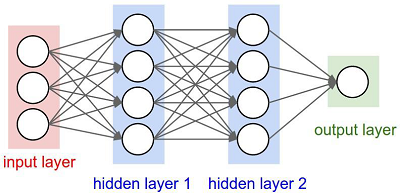
\includegraphics[width=\linewidth]{CNNbasicarch.png}
  \caption{NN Basic Architecture}
  \label{fig:NN Basic}
\end{figure}

\paragraph{•}
Figure 1 depicts a conceptual overview of the NN. CNN consists of four core layers including an input layer, two hidden layers, and an output layer. The difference between Neural network and CNN is the parameter sharing. That is CNN shares parameters where as i NN, the parameters are used only once. Hence performance of CNN is better interms of efficiency and memory power. A CNN could consists of many layers that can be used repeatedly to form a Deep Neural Network [1]. We provide definitions for some of the commonly used layers in the CNN [1].  
1. Input Layer: This layer carries the information for the raw pixel values that represent an image. 
2. Convolutional Layer: This layer obtains results from the neuron layer that is connected to the input region. This layer is defined with the specific number of filters to be used. Each filter could be based on a 5x5 window that slides over the input data and gets the pixel with the maximum intensity as the output [10]. 
3. Rectified Linear Unit(ReLU) Layer: The ReLU layer features an element wise activation function on the image data [10]. A CNN uses back propagation. We apply the ReLU function to preserve the identical values of the pixels and resist from being changed by the back propagation. 
4. Pooling Layer: The pooling layer performs a down-sampling operation along the width and height [10]. 
5. Fully Connected Layer: This layers computes the score classes and determines the class that has the maximum score corresponding to the input digits [10]. 
 
\subsubsection{Extraction of a Feature: }
All neurons associated with a feature are assigned with a same weight. This assignment ensures that all neurons detect the same feature at different positions in the input image [1]. 
\paragraph{•}
The CNN features Subsampling Layer that reduces the spatial resolution of each feature map. The “subsampling” typically refers to as a desirable act of reducing the overall size of a signal. This layer reduces the effect of noise and associated distortion invariance. 
\paragraph{•}
The CNN also features Max Pooling process that preserves the locations on the image that shows the strongest correlation to each feature (i.e., the maximum value). These maximum values combine together to form a lower-dimensional output and it provides a form of translation invariance. This process can be visualized as a cascading of max-pooling layer with a convolutional layer [14-16].

 
 
\subsection{CNN for Handwritten Digit Recognition }
The CNN facilitates the recognition of the handwritten digits in a form of the three main phases [1]. 
\paragraph{•}
\begin{figure}
  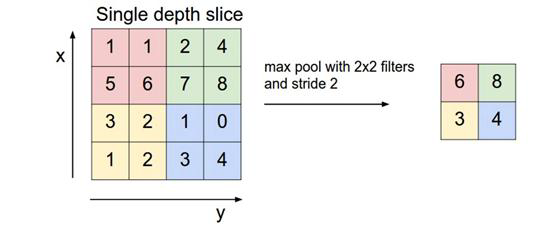
\includegraphics[width=\linewidth]{Pooling.png}
  \caption{Pooling.}
  \label{fig:Pooling}
\end{figure}

\paragraph{1. Input MNIST Data:}
  (see fig: Pooling) The first phase facilitate the input of the MNIST data in the form of a 784-d array of pixels. Therefore, the data is converted to grayscale images representing 28x28 matrix of pixels. 
\paragraph{2. Building Network Architecture:}
  The second phase defines the models used to build a CNN. The current study uses the Sequential class from Keras to build the network. This network features three sets of layers “CONV =>ReLU=> POOL”. 
\paragraph{•}
First Convolution Layer: The first layer receives convolutional filters that go as a sliding window of size 5x5 over all the images of 28x28 matrix size. This layer gets the pixels with most intensity value. ReLU Function uses convolution method that uses Back Propagation. So using the ReLU function as the activation function just after the convolutional layer reduces the likelihood of the vanishing gradient and avoids sparsity. This way we don’t lose the important data and even get rid of redundant data like a lot of 0‟s in the pixels. c) Pooling Layer: The pooling layer gets the data from the ReLU function and down-samples the steps in the 3D tensor. In short it pools all the pixels obtained from previous layers and again forms a new image matrix of a smaller size. These images are again input into the second set of layers i.e. “CONV =>ReLU=> POOL” and this process goes on till we get to a smallest set of pixels from which we can classify the digit. 
\paragraph{3. Fully Connected Layer: }
The fully connected layer is used to connect each of the previous layers to the next layers. This layer consists of 500 neurons. Finally, we apply a SoftMax/Sigmoid Classifier that returns a list of probabilities for each of the 10 class labels. The class label with the largest probability is chosen as the final classification from the network and shown in the output. 
\paragraph{•}
This output received is used to make the confusion matrix for the model. In this we can add more number of layers but adding more layers might affect the accuracy of the system. Since, it uses multiple layers,  it is called as a Deep Learning system.(see fig:Softmax)
\begin{figure}
  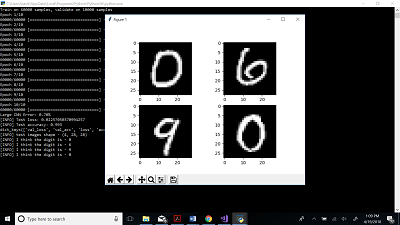
\includegraphics[width=\linewidth]{softmax.png}
  \caption{softmax.}
  \label{fig:softmax}
\end{figure}


\section{Results And Analysis }
\label{gen_inst}

\subsection{Analysis}

\begin{table}[ht]
\begin{center}
\caption{CNN Model Results} % title of Table
\centering 
 	 \label{CNN-table}
 	 \centering
    \begin{tabular}{ | l | l | l | p{5cm} |}
    \hline
    CNN & Accuracy & Error rate & Test Loss \\ \hline
    Relu Softmax & 99.3 & 0.70 & 0.02257. \\ \hline
    ReLu Sigmoid & 99.08 & 0.92 & 0.02769 \\ \hline    
    \end{tabular}
\end{center}

\end{table}


\paragraph{Model Validation}
An extensive set of modeling runs suggest that the CNN model can process a given image of handwritten digit, feeding it to the network, and predict the digit in an accurate manner. Figure 5 shows the sample results that validate the accuracy of the predictions from the developed model. For example, the user inputs the handwritten images of '3' and '2' and the CNN model recognizes the numbers accurately. The author did not observe a single instance where the CNN model failed to prediction a given image of handwritten letter.



\begin{figure}
  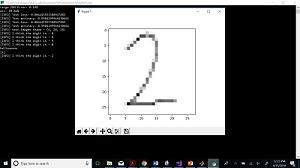
\includegraphics[width=\linewidth]{HRimg2.png}
  \caption{HRimage2.}
  \label{fig:HRimage2}
\end{figure}


\paragraph{•}

Implementation of CNN using ReLu and Sigmoid activation functions gives the maximum accuracy when compared with ReLu and Sigmoid activation functions(see Table1). While the CNN presents a complex code and higher  processing time when compared with normal Machine Learning algorithms, it offers higher accuracy. Note that these analysis details are for training and testing on the CPU only. Using GPU for this purpose can greatly reduce the training and testing time.
\begin{figure}
  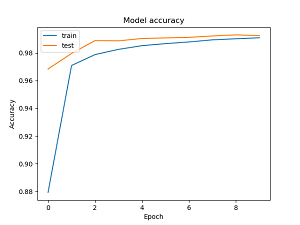
\includegraphics[width=\linewidth]{CNNAccuracy.png}  
  \caption{Accuracy.}
 \end{figure}

\paragraph{Conclusion}
Digit recognition is an excellent prototype problem for learning about neural networks and it gives a great way to develop more advanced techniques of deep learning. 
Digit recognition is an excellent prototype problem for learning about capabilities of neural networks and it provides new ways for developing advanced deep learning techniques. The author plans to explore and use the CNN for identifying bacteria in biofilm images [17].

\paragraph{•}
The commercial applications require accurate that the model recongize the digits and characters in an accurate manner without reducing the speed of recognition. We demonstrate that the CNN with 3 hidden layers gives the most amount of accuracy of 99.24% (with ‘Softmax’ and Relu activation functions). 

\paragraph{•}
The proposed study demonstrates that the deep learning concepts can open new ways for digitalization. While this study focused on recognition of the digits,  it can be extended to letters and also for recognizing a person’s handwriting. This can eliminate the need for typing. People can write  in their own handwriting and then convert it in digital form by just clicking their pictures. Digit recognition is an excellent prototype problem for learning about neural networks and it leads new ways for developing advanced deep learning techniques.

\section{References:}


1. Dutt, A. and A. Dutt, Handwritten Digit Recognition Using Deep Learning. International Journal of Advanced Research in Computer Engineering and Technology, 2017. 6(7): p. 990-997.

2.	Jain, N., et al., Hand Written Digit Recognition using Convolutional Neural Network (CNN). 2017.

3.	Subhashini, V.P.P., Hand Written Digit Recognition using Kalman Filter.

4.	ABINAYA, A., et al., Detection and Classification of Brain Tumor Using SVM And K-NN Based Clustering.

5.	Albeahdili, H.M., A.A. Haider, and N.E. Islam, Robust Convolutional Neural Network for Image Recognition. International Journal of Advanced Computer Science and Applications, 2015. 6(11): p. 105-111.

6.	Lauer, F., C.Y. Suen, and G. Bloch, A trainable feature extractor for handwritten digit recognition. Pattern Recognition, 2007. 40(6): p. 1816-1824.

7.	Hamid, N.A. and N.N.A. Sjarif, Handwritten Recognition Using SVM, KNN and Neural Network. arXiv preprint arXiv:1702.00723, 2017.

8.	Retreived from http://yann.lecun.com/exdb/mnist/, 4/21/2018.

9.	Retreived from https://en.wikipedia.org/wiki/Supportvectormachine, 04/21/2018.

10.	Retreived from http://cs231n.github.io/convolutional-networks/,  4/21/2018.

11.	Meng, W., A sentence-based image search engine. 2015.

12.	Retreived from http://www.deeplearningbook.org/lectureslides.html,  4/21/2018.

13.	Retreived from http://yann.lecun.com/exdb/lenet/,  4/21/2018.

14.	Retreived from https://www.cedar.buffalo.edu/~srihari/CSE676/index.html , 4/21/2018.

15.	Retreived from https://cs231n.stanford.edu/slides/2017/cs231n2017lecture6.pdf,  4/21/2018.

16.	Retreived from https://machinelearningmastery.com,  4/21/2018.

17.	Vyas, N., et al., A quantitative method to measure biofilm removal efficiency from complex biomaterial surfaces using SEM and image analysis. Scientific reports, 2016. 6: p. 32694.

  
\end{document}
